\documentclass{article}
\usepackage[utf8]{inputenc}
\usepackage{lmodern}
\usepackage{titlesec}
\usepackage{listings}
\usepackage{xcolor}
\usepackage{minted}
\usepackage{graphicx}
\usepackage{multicol}
\usepackage{lipsum}
\usepackage{scrextend}
\usepackage{pdfpages}
\usepackage{hyperref}

\graphicspath{{img/}}

\titlespacing*{\section}      {0em}{1.25em}{.75em}
\titlespacing*{\subsection}   {0em}{1em}{.5em}
\titlespacing*{\subsubsection}{0em}{.75em}{.5em}
\titlespacing*{\paragraph}    {0em}{.50em}{.5em}
\setlength\parindent{0pt}
\setlength{\parskip}{1mm}

\newcommand{\newlineparagraph}[1]{\paragraph{#1}\mbox{}\\}
\newcommand{\twodashes}{\texttt{-{}-}}

\colorlet{punct}{red!60!black}
\definecolor{delim}{RGB}{20,105,176}
\colorlet{numb}{magenta!60!black}

\lstset{
    basicstyle=\normalfont\ttfamily,
    showstringspaces=false
}

\begin{document}
    \begin{titlepage}
       \begin{center}
            \vspace*{1cm}
    
            \huge
            \textbf{Netzwerk‐basiertes RobotGame mit zentralem Server}
        \end{center}
    
        \vspace{1.5cm}
        \begin{addmargin}[8em]{0em}
            \Large
            Name: Michael Domanek\par
            Klasse: 5BHIF\par
            Katalognummer: 4\par
            Beispielnummer: 35
        \end{addmargin}
        
        \vfill
        
        \begin{center} 
        
\includegraphics[width=\textwidth]{Robocode}
                
        \end{center}
    \end{titlepage}

\newpage

\tableofcontents

\newpage

\section{Aufgabenstellung}
Netzwerk‐basiertes RobotGame wie robowiki mit zentralem Server.

\section{Hintergrund}

Robocode ist ein Spiel, bei dem das Ziel darin besteht, einen Roboter zu programmieren, der gegen andere Roboter antritt. Der Spieler hat keinen direkten Einfluss auf das Spielgeschehen, sondern programmiert die KI des Roboters und gibt vor, wie er sich verhalten soll und auf Ereignisse reagieren soll. 

Ürsprünglich war Robocode gedacht Kindern bzw. Anfängern spielerisch die Programmiersprache Java beizubringen. In der Sprache wurde auch das Spiel geschrieben und unterstützt dadurch auch alle gängigen Betriebssystemen(Windows, macOS, Linux, ...)

\subsection{Geschichte}
Matthew A. Nelson hat im Jahr 2000 begonnen das Spiel zu entwickeln . Das Projekt hat zuerst als persönlicher Freizeitprojekt gestartet und 2001 hat er es professionell für IBM gemacht. 2005 wurde es dann Open Source, aber die  Weiterentwicklung wurde gestoppt. Viele Programmierer haben zu dem Projekt RobocodeNG, das von Flemming N. Larsen geleitet wurde beigetragen und Erweiterungen hinzugefügt und Bugs gefixt. 2006 wurden das Projekt dann als Version 1.1 mit dem offiziellen Robocode Projekt zusammengefügt. Seit dem gibt es immer wieder neue Versionen.

\subsection{Installation}

Das Spiel ist ein Java-Programm das man sich herunterladen kann. Dann kann man seinen ersten Roboter programmieren mit Hilfe der Robowiki. Danach kann dann seinen Roboter gegen andere einfache Beispielroboter antreten lassen. Wenn man gegen alle Roboter gewonnen hat, kann man sich bessere Roboter aus dem Internet herunterladen. Es gibt auch Tuniere in dene die besten Roboter antreten und viele der besten Roboter stehen auch zum Download zur Verfügung.

\begin{figure}[h]
    \centering
    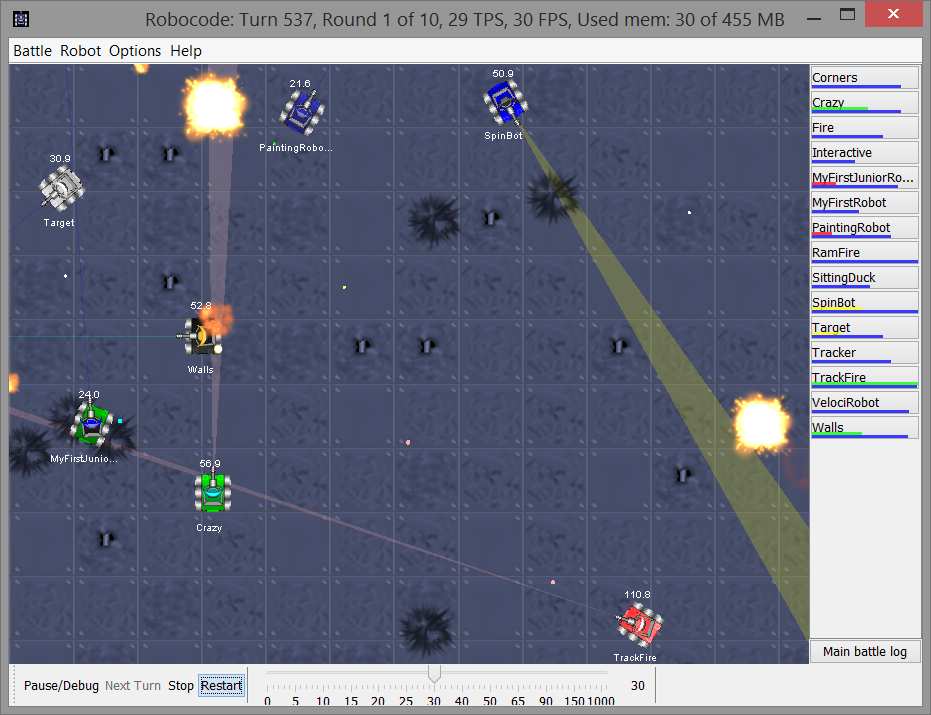
\includegraphics[width=\textwidth]{Robocodegame}
    \caption{Screenshot aus dem originalem Spiel}
\end{figure}

\subsection{Spieleigenschaften}

Jeder Roboter besteht aus einem Untergestell, einer Waffe und einem Radar. Beim fahren bewegt sich alles. Beim Rotieren kann man das Untergestell, die Waffe und das Radar unabhängig voneinander bewegen. Die Waffe ist natürlich um andere Roboter abzuschießen. Das Radar um andere Roboter zu finden.

Das Spiel verwendet das Kartesische Koordinatensystem, das heißt (0, 0) ist unten links. Die Rotation des Roboters ist natürlich 360° und 0° ist im Norden. 

Die Beschleunigung des Roboters ist 1 Pixel/Runde und die Verlangsamung ist 2 Pixel/Runde. Die maximale Geschwindigkeit beträgt 8 Pixel/Runde.

Jeder Roboter startet am Anfang mit einer 100\% Energie.  
Der Roboter verliert jedes Mal Energie, wenn er gegen eine Wand fährt, wenn er von einer gegnerischen Kugel getroffen wird, wenn er einen Gegner rammt oder gerammt wird oder wenn er sein Waffe abfeuert. Er bekommt Energie zurück wenn er einen anderen Roboter abschießt, zerstört oder rammt.

Das Spießen funktioniert so das man entscheiden kann wie viel Schaden die Kugel machen wird. Desto mehr Schaden desto langsamer fliegt die Kugel und sie kostet dann auch mehr Energie. Man muss auch länger warten bis man wieder Schießen kann. Vor allem wenn man wenig Energie hat sollte man eine niedrige Feuerkraft wählen.

Wenn man einen anderen Roboter rammt, bekommen beide Schaden, aber der Rammende bekommt Energie zurück. Wenn man gegen eine Wand fährt bekommt man auch Schaden.

\subsection{Spielende und Gewinner}

Der Gewinner des Spiels ist nicht der letzte Überlebende sonder der mit den meisten Punkten. Punkte kann man erhalten folgendermaßen erhalten:

\begin{itemize}
\item Survival Score - wenn jemand stirbt bekommen alle Lebenden Punkte
\item Last Survivor Bonus - wenn man der letzte Überlebende ist
\item Bullet Damage - wenn man Gegner abschießt
\item Bullet Damage Bonus - wenn man einen Roboter zerstört beim Abschießen 
\item Ram Damage - wenn man eien Gegner rammt
\item Ram Damage Bonus - wenn man einen Roboter zerstört beim Rammen 
\item 1sts, 2nds, 3rds - wenn man erste, zweiter oder dritter wird
\end{itemize}

\subsection{Programmierung}
Die Programmierung des Roboters ist grundsätzlich Eventbasiert. Am Anfang jeder Runde wird die Methode \textit{run()} aufgerufen. Dort wird die Initialisierung des Roboters durchgeführt. Man kann sein Aussehen also die Farbe festlegen und das grundsätzliche Verhalten des Roboters. Man kann auch in einer Endlosschleife, das Verhalten des Roboters bestimmen. In dieser Schleife kann man mit get-Methoden den Zustand des Roboters abfragen und dann das Verhalten des Roboters verändern.

Man kann auch auf viele Events reagieren, die während des Spiels passieren. Events sind zum Beispiel onScannedRobot(event) und onHitByBullet(event) auf die man reagieren kann. Durch diese Events kann man auch auf die Endlosschleife in der Initialisierung verzichten.

\subsection{Spielmodi und Challenges}
Es gab auch viele Robocode Wettbewerbe. In dieses sogenannten Challenges werden die besten Roboter bzw. Programmierer in einem bestimmten Spielmodus gesucht. Ein Bespeil ist die Movement Challenge 2K7.

Es gibt neben dem normalen Spielmodus auch noch viele weitere Spielmodi wie zum Beispiel 1v1, Melee, Teams Twin Duel Es gibt auch Wettbewerbe mit maximaler Codegröße namens MiniBots, MicroBots, and NanoBots.

\vspace{1.5cm}

\section{UML}

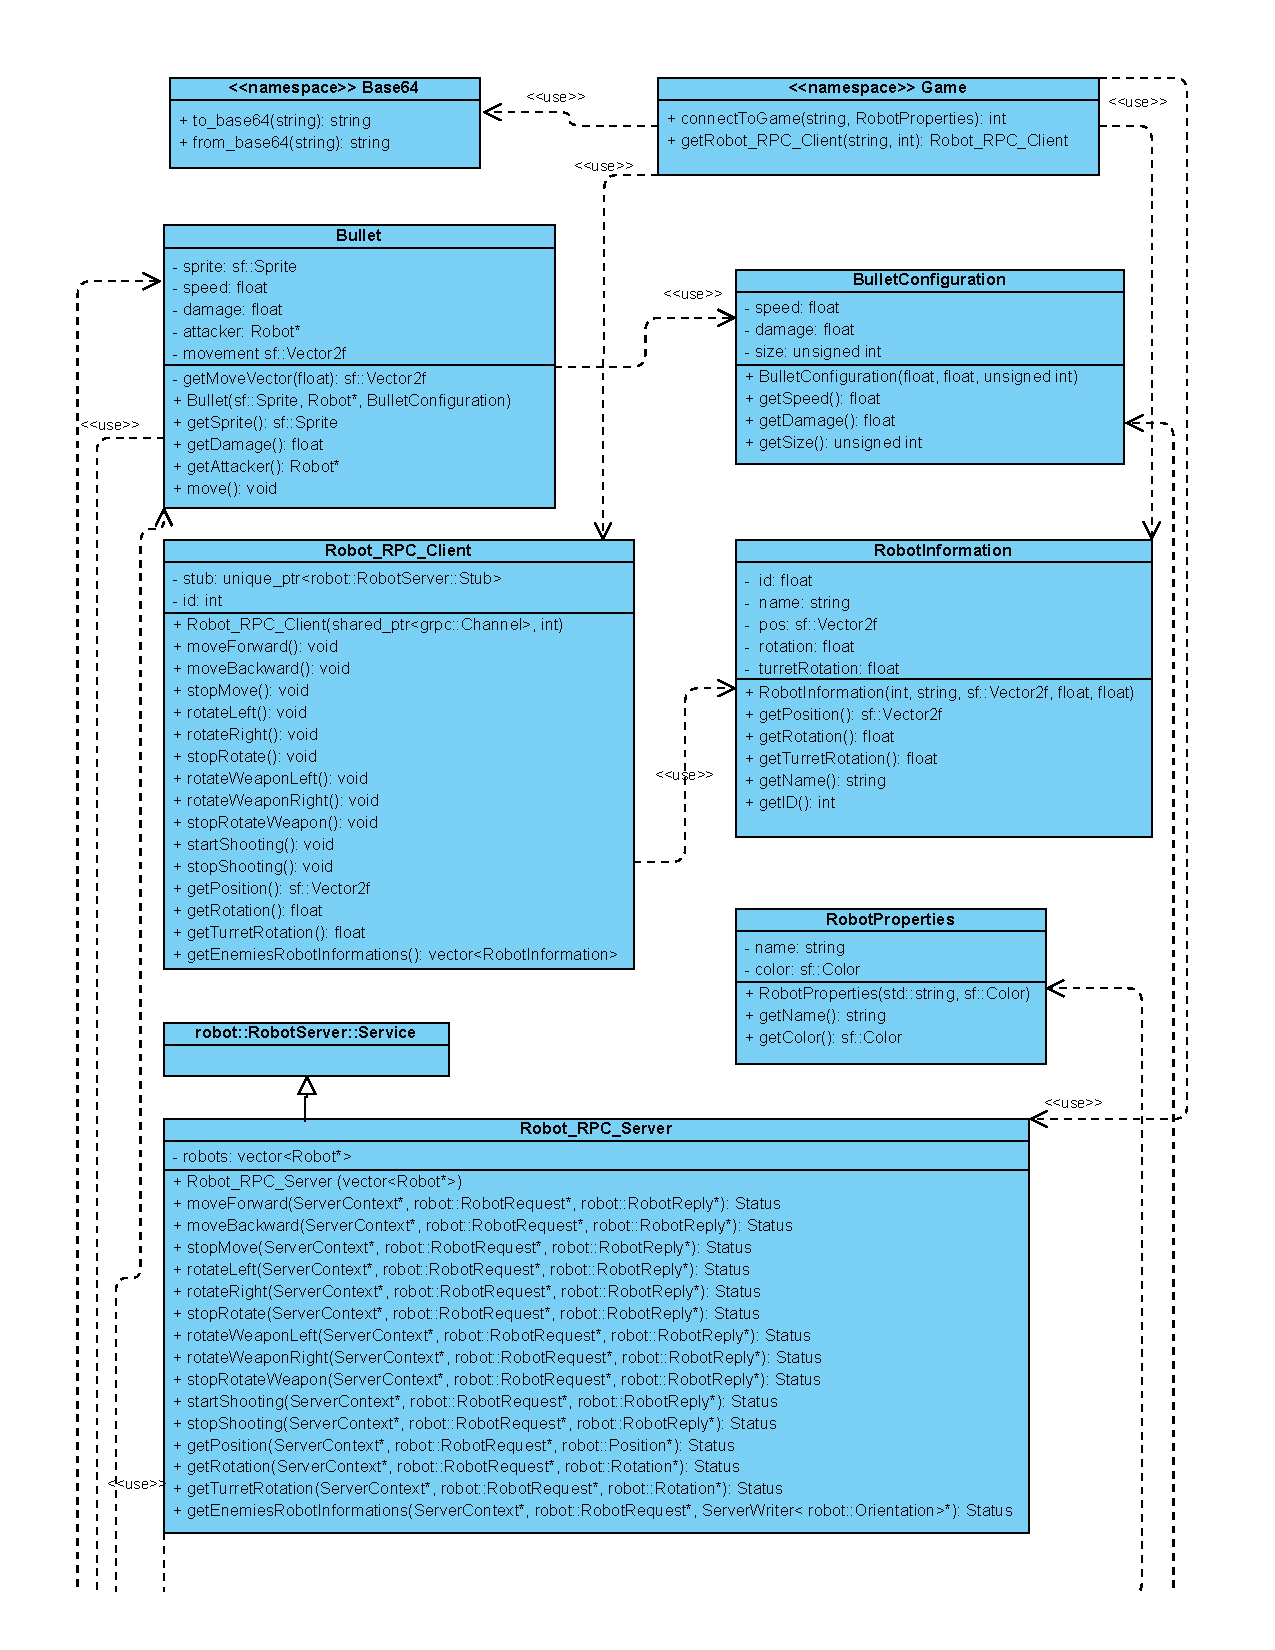
\includepdf[pages=-]{UML.pdf}


\section{Umsetzung}

\subsection{Spiel Idee}
Die Idee meines Spieles ist es das man keine Events verwendt. Stattdessen man alle Information über den grpc Server / Cliet erhält und auch sendet. Man kann keine anderen Roboter rammen und bekommt auch keinen Schaden an Wänden. Man bekommt auch keine negative Effekt wenn man schießt und die Feuerkraft ist immer gleich. Außerdem gibt es keinen Radar. Jeder Roboter kann alles über andere Roboter abfragen. Der Rest ist sehr ähnlich zu dem original.

Die Idee meines Spiels ist das man zuerst den Server startet. Dieser hat viele Optionen die ich später noch beschreibe. Danach können sich die Clients verbinden und legen ihren Namen und die Farbe des Roboters fest. Nach dem sich alle Clients verbunden habe bekommen die Clients die Spieleinstellungen also die Roboterkonfiguration. Jetzt können sie sich mit dem Robot\_RPC\_Client verbinden. Ab jetzt können sie folgende Methoden aufrufen um ihren Roboter zu steuern oder Informationen über den eigenen oder die anderen Roboter zu bekommen.

\begin{minted}[linenos=false]{c++}
void moveForward();
void moveBackward();
void stopMove();

void rotateLeft();
void rotateRight();
void stopRotate();

void rotateWeaponLeft();
void rotateWeaponRight();
void stopRotateWeapon();

void startShooting();
void stopShooting();

sf::Vector2f getPosition();
float getRotation();
float getTurretRotation();
std::vector<RobotInformation> getEnemiesRobotInformations();
\end{minted}

Der Server funktioniert so, dass er zuerst gestartet werden muss, da er auf alle Clients wartet. Danach erstellt er die Roboter, der Clients die sich verbunden haben. Sobald sich alle verbunden haben erstellt er das Spiel mit allen Optionen und es öffnet sich auch das GUI des Spiels. Dann wird der Grpc-Server gestartet. Die Clients werden Informiert und das Spiel geht los. Die Roboter spawnen immer in einer Ecke und zeigen fast in die Mitte gerade so das sie noch aneinander vorbeischießen. Während des Spiels werden folgende Aktionen durchgeführt:

\begin{itemize}
\item Roboter wird bewegt, gedreht und die Waffe gedreht
\item Roboter schießt
\item Bullets werden bewegt
\item Es wird überprüft ob die Kugel getroffen hat
\item Die GUI wird upgedated (alles wird gezeichnet)
\end{itemize}

\begin{figure}[h]
    \centering
    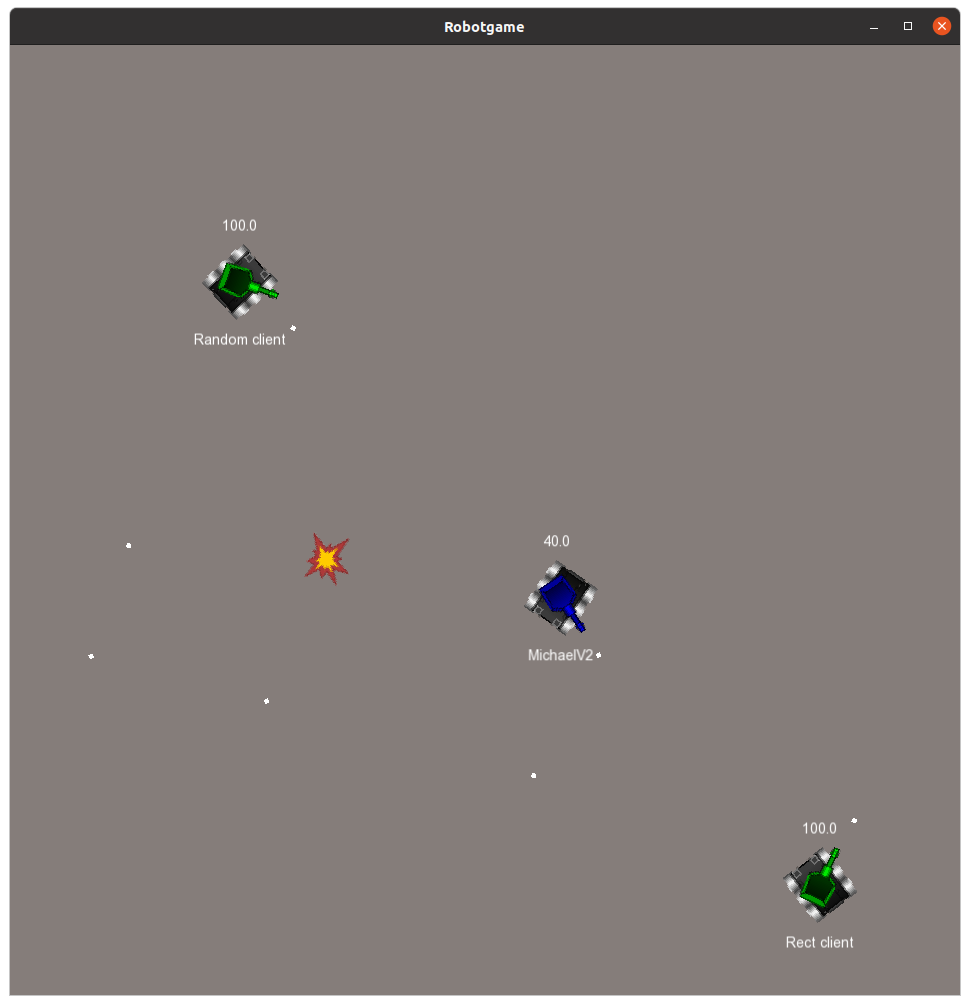
\includegraphics[width=\textwidth]{Robotgame}
    \caption{Screenshot aus meinem Spiel}
    \label{fig:screenshot}
\end{figure}

\pagebreak

\subsection{Serveroptionen}
\begin{figure}
    \centering
    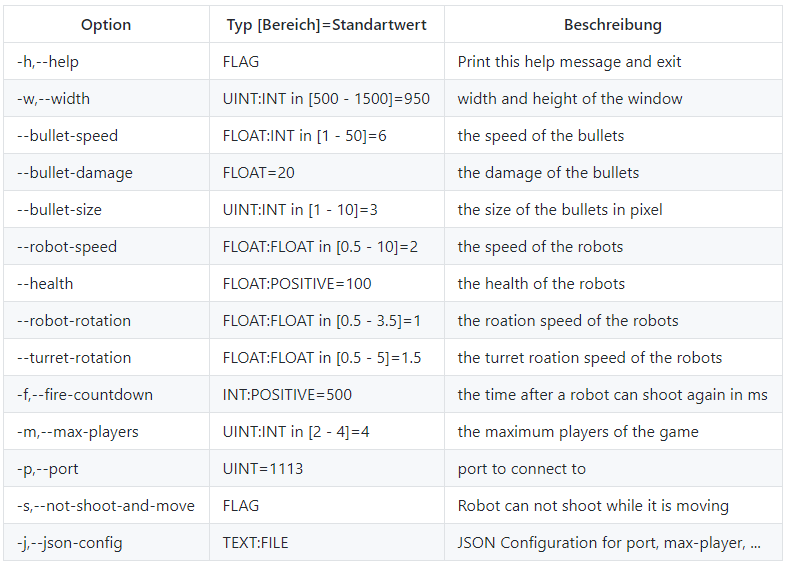
\includegraphics[width=\textwidth]{Serveroptionen}
    \caption{Serveroptionen}
    \label{fig:screenshot}
\end{figure}

In diesem Kapitel geht es um die Einstellungsmöglichkeiten des Servers.

\subsubsection{width}

Die Breite und Höhe des Fensters der GUI kann verändert werden. Das Fenster ist immer ein Quadrat. Die Größe muss zwischen 500-1500 pixel sein.

\subsubsection{bullet-speed}

Die Geschwindigkeit des Geschosses der Waffe kann verändert werden. Die Kugel kann sehr langsam oder sehr schnell fliegen, also sozusagen direkt treffen wenn die Waffe auf einen Roboter gerichtet ist.

\subsubsection{bullet-damage}

Der Schaden der Waffe kann beliebig gewählt werden.

\subsubsection{robot-speed}

Die Geschwindigkeit mit der sich der Roboter bewegt.

\subsubsection{health}

Die Start-Leben des Roboters.

\subsubsection{robot-rotation}

Die Geschwindigkeit mit der sich der Roboter drehen kann.

\subsubsection{turret-rotation}

Die Geschwindigkeit mit der sich die Waffe des Roboters drehen kann.

\subsubsection{fire-countdown}

Die Zeit nach dem der Roboter erneut schießen kann. Eine niedrige Abklingzeit bedeutet das der Roboter sehr schnell schießt, fasst wie ein Maschinengewehr. Hohe Abklingzeit heißt das er sehr selten schießen kann und daher die Treffergenauigkeit wichtiger ist.

\subsubsection{max-players}

Die maximale Anzahl der Spieler bzw. der Clients, die sich verbinden könnnen. Es müssen mindestens 2 Spieler sein also ein 1 gegen 1 und es können maximal 4 Spieler sein.

\subsubsection{port}

Der Port der asio-Verbindung

\subsubsection{not-shoot-and-move}

Eine Flag, ob der Roboter schießen kann während er sich bewegt. Das heißt er darf nicht fahren und sich nicht drehen bzw. die Waffe darf sich auch nicht drehen.

\subsubsection{json-config}

Port, max-players und not-shoot-and-move kann 

\pagebreak

\section{Verwendung}

Die normale Verwendung ist wie folgt. Es wird zuerst der Server gestartet. Es können auch eine Vielzahl an Optionen übergeben werden wie gerade beschrieben.

Danach startet man 4 Clients jeweils in einem eigenen Terminalfenster. Ich hab 4 Beispielclients implementiert. Der Fortgeschrittenste ist domanekV2. Diese berechnet sich die kürzeste Distanz zum nähesten Roboter und schießt diesen dann ab und verfolgt ihn mit seiner Waffe (er ziehlt immer auf ihn). Der Rect-client fährt in einem großen Rechteck im Feld immer wieder im Kreis und dreht die Waffe dauerhaft im Kreis und schießt. Der Random client fährt semi-random im durch das Feld und schießt irgendwohin.

\begin{lstlisting}

./robo-server

./rect-client
./random-client
./domanek
./domanekV2

\end{lstlisting}

Der einfachste Weg das Programm zu testen ist den Server mit 2 Spielern zu starten. Der test-client führt einfach jede mit einem Abstand von einer Sekunde aus und gibt dann alle Informationen über den Roboter und die Gegner, die er über den Server erhalten kann, aus. Am Anfang werden noch die Spieleinstellungen (RobotConfiguration) ausgegeben.

\begin{lstlisting}

./robo-server -m 2

./test-client
./test-client
\end{lstlisting}


\section{Code-Beispiele}
Der Grpc-Server wird folgendermaßen gestartet. Es wird mit dem Robot\_RPC\_Server Service erstellt, der die Requests der Clients bearbeitet. Der Server läuft bis er am Ende des Spiels heruntergefahren wird.

\begin{minted}[linenos=false]{c++}
Robot_RPC_Server service{robots};
grpc::ServerBuilder builder;
builder.AddListeningPort("0.0.0.0:50051", grpc::InsecureServerCredentials());
builder.RegisterService(&service);
std::unique_ptr<grpc::Server> server(builder.BuildAndStart());

std::thread grpcServerThread{[&server]{
    server->Wait();
}};
grpcServerThread.detach();
\end{minted}

\vspace{1cm}

Der Grpc-Service von moveForward sieht folgendermaßen aus. Es wird die ID des Roboters, der sich bewegen will an den Server geschickt. Der Client speichert sich beim Initialisieren die Client-ID und sendet sie dem Server. Der Server führt die Methode beim Roboter aus, da er eine Referenz des vectors mit allen Robotern hat.
Der Client bekommt keinen response, lieft aber einen Fehler wenn die Kommunikation nicht funktioniert hat. Der Server erbt von dem RobotServer::Service, dieses wird anhand des service aus dem proto file erstellt und enhält die virtuellen Methoden, die implementiert werden müssen.

Bei anderen Methoden die etwas zurückliefern wird statt der leeren RobotReply, einen Nachricht mit Inhalt als reply zurückgeliefert. z.B. reply.set\_x(). Die Client-Implementierung liest das dann aus und gibt dem Client das richtig Objekt zurück.

\begin{minted}[linenos=false]{c++}
//Protobuf
rpc moveForward (RobotRequest) returns (RobotReply) {}
message RobotRequest {
    int32 id = 1;
}

message RobotReply {}


#include <grpcpp/grpcpp.h>
#include "robotServer.grpc.pb.h"

//Client
std::unique_ptr<robot::RobotServer::Stub> stub;
Robot_RPC_Client(std::shared_ptr<grpc::Channel> channel, int id) :
    stub(robot::RobotServer::NewStub(channel)), id(id) {}

void Robot_RPC_Client::moveForward() {
    ClientContext context;
    RobotReply reply;
    RobotRequest request;
    request.set_id(id);

    Status status = stub->moveForward(&context, request, &reply);

    if (!status.ok()) {
        throw std::runtime_error(status.error_code() + ": " + status.error_message());
    }
}


//Server
std::vector<Robot*> robots;
Robot_RPC_Server (std::vector<Robot*>& robots) : Service(), robots(robots) {}

Status Robot_RPC_Server::moveForward(ServerContext* context, const RobotRequest* request,
                                     RobotReply* reply) {
    (void) context;
    (void) reply;
    
    robots[request->id()]->moveForward();

    spdlog::debug("Robot {}: moveForward", request->id());

    return Status::OK;
}
\end{minted}

Der Client erstellt den Client folgendermaßen. Er übergibt den Port und die ID und ruft dann die Methode aus. moveForward() lieft nichts zurück, getPosition() liefert einen sf::Vector2f.

\begin{minted}[linenos=false]{c++}
#include "robotClient.h"

Robot_RPC_Client robotClient = Game::getRobot_RPC_Client(grpcPort, id);

robotClient.moveForward();

sf::Vector2f pos{robotClient.getPosition()};
fmt::print("x: {} | y: {}\n", pos.x, pos.y);

\end{minted}

Die Implementierung von move(), rotate() und rotateWeapon() ist sehr ähnlich. Ich beschreibe sie anhand von rotate(). Die Funktion wird einmal pro Durchgang aufgerufen und dreht den Roboter abhängig von rotateSign. Rotatesign kann -1, 0 und 1 sein. -1 bedeutet nach links drehen, 0 bedeutet nicht drehen und 1 bedeutet.
Die Methoden rotateLeft(), rotateRight() und stopRotate() ändern lediglich den Wert des chars (char da es der kleinste Datentyp für -1, 0 und 1 ist). Diese Methoden werden auch von dem grpc-Server verwendet. Die Besonderheit von rotate() ist noch, dass sie auch die Waffe mitdreht und das überprüft werden muss ob sie die Robter berührennach dem drehen und dann kann sich nicht gedreht werden.

Am Ende der Drehung muss noch der Movement-vector neu berechnet werden, der entscheidet in welche Richtung der Roboter fährt.

shoot() hat nur 2 optionen schießen und nicht schießen und ist daher ein boolean.

\begin{addmargin}[-3em]{0em}

\begin{minted}[linenos=false]{c++}
char rotateSign{};

void Robot::rotate() {
    const float robotRotation{config.getRobotRotation()};
    robot.setRotation(robot.getRotation() + (robotRotation * rotateSign));
    turret.setRotation(turret.getRotation() + (robotRotation * rotateSign));

    if (rotateSign) {
        for(Robot* robo: window.getRobots()) {
            if (this != robo && robot.getGlobalBounds().intersects(robo->getGlobalBounds())) {
                robot.setRotation(robot.getRotation() + (robotRotation * -rotateSign));
                turret.setRotation(turret.getRotation() + (robotRotation * -rotateSign));
                break;
            }
        }

        movement = getMoveVector();
    }
}

void Robot::rotateLeft() {
    rotateSign = -1;
}

void Robot::rotateRight() {
    rotateSign = 1;
}

void Robot::stopRotate() {
    rotateSign = false;
}
\end{minted}

\end{addmargin}

Der movment-vector, also wohin der Roboter beim vorwärtsfahren fährt, wird einfach anhand der Rotation des Roboters und der Fahrgeschwindigkeit berechnet.

\begin{minted}[linenos=false]{c++}
sf::Vector2f Robot::getMoveVector() {
    const float angle{robot.getRotation() * (float)M_PI / 180.0f};
    const float speed{config.getSpeed()};
    return sf::Vector2f{sin(angle) * speed, cos(angle) * -speed};
}
\end{minted}

Etwas anzuzeigen ist in SFML einfach. Am Anfang wird die ganze Fläche gecleart. Dann werden die erstellten Sprite bzw. Text einfach an die Methode draw() übergeben. Am Ende werden alle diese Objekte dann durch die Methode display() gezeichnet.

\begin{minted}[linenos=false]{c++}
window.clear();

for(Robot* robot: robots) {
    window.draw(robot->getRobotSprite());
    window.draw(robot->getTurretSprite());
    window.draw(robot->getNameText());
    window.draw(robot->getHealthText());
}

window.display();
\end{minted}


\section{Quellen}

Hintergrund - Robowiki
\begin{itemize}
\item \url{https://robowiki.net/wiki/Main_Page}
\item \url{https://robowiki.net/wiki/Robocode/Getting_Started}
\item \url{https://robowiki.net/wiki/Robocode/FAQ}
\item \url{https://robowiki.net/wiki/Robocode/My_First_Robot}
\item \url{https://robowiki.net/wiki/Robocode/Game_Physics}
\item \url{https://robowiki.net/wiki/Robocode/Robot_Anatomy}
\item \url{https://robowiki.net/wiki/Robocode/Scoring}
\end{itemize}
stream-basierte Kommunikation mit asio:
\begin{itemize}
\item 26\_tcpip\_programming1 Seite 16-17
\end{itemize}

\end{document}



